\question %8
\emph{Implémentez sous MATLAB ce modèle linéaire continu,
et calculez la solution correspondant aux données fournies sur icampus.
Commentez l'allure de la solution obtenue, et comparez à la solution du modèle
simplifié. Commentez également l'intégralité des variables de la solution ;
celle-ci présente-t-elle un aspect problématique ?}

\begin{figure}[H]
  \begin{center}
    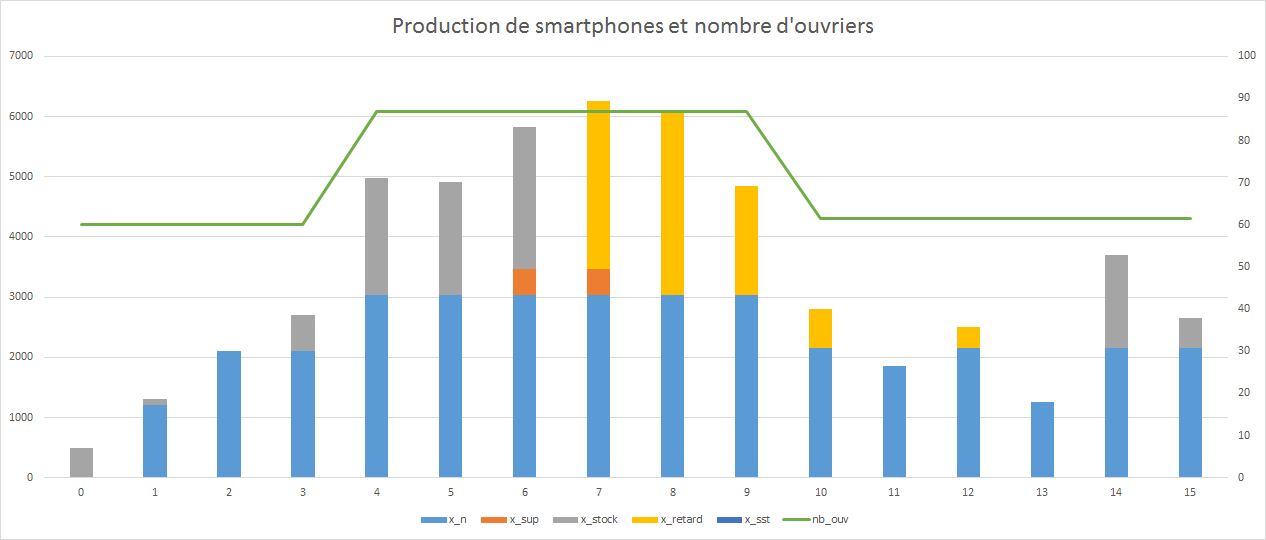
\includegraphics[scale = 0.75]{img/grapheProductionOuvNonInt.png}
	  \caption{Répartition du moyen de production des smartphones en fonction des semaines et évolution du nombre d'ouvriers dans le cas non entier.}
	  \label{fig:grapheProductionOuvNonInt}
  \end{center}
\end{figure}